\documentclass[10pt, aspectratio=169]{beamer}

\usepackage{svg}
\usepackage[absolute,overlay]{textpos}
\usepackage{fontspec}
\usetheme[progressbar=foot]{metropolis}
\setbeamercolor{background canvas}{bg=white}

\setbeamertemplate{section page}{
    \begin{minipage}{\textwidth}
        \centering
        \usebeamercolor[fg]{section title}
        \usebeamerfont{section title}
        \textsc{\insertsection}\par
        \vspace{1cm}
    \end{minipage}
    \begin{minipage}{\textwidth}
        \usebeamercolor[fg]{normal text}
        \tiny\tableofcontents[currentsection]
    \end{minipage}
}

\usepackage{hyperref}
\hypersetup{
    colorlinks = true,
    urlcolor = blue,
    linkcolor = black
}

\usepackage[scale=1]{ccicons}

% Code listings
\usepackage{minted}
\usepackage{caption}
\usepackage{xcolor}
% New command that includes caption with the file path
\captionsetup[listing]{labelformat=empty}
\newcommand{\inputmintedpath}[2]{
  \begin{listing}[H]
    \inputminted[
      linenos,
      numbersep=15pt,
      framesep=2mm,
      bgcolor=lightgray!20,
      baselinestretch=1.1,
      fontsize=\scriptsize,
      firstnumber=1,
      stepnumber=5,
    ]{#1}{#2}
    \caption{\scriptsize\texttt{\detokenize{#2}}} % Caption (file path)
  \end{listing}
}

\setbeameroption{hide notes} % Only slides
%\setbeameroption{show only notes} % Only notes
%\setbeameroption{show notes on second screen=right} % Both
% Add notes like this: \note{Note}

% Make surethat parskip is properly adjusted also in columns
\renewcommand{\baselinestretch}{1.3}
\makeatletter
\newcommand{\@minipagerestore}{\setlength{\parskip}{0.65em}}
\makeatother

\metroset{titleformat frame=smallcaps}
\newcommand{\parspace}{\vspace{1em}}


\title{Hands-on Zephyr Project Workshop}
\subtitle{Navigating Low Power IoT Development with Practical Examples}
\author{Jonas Remmert}
\institute{IoT Embedded Systems Engineer at Phytec Messtechnik GmbH}
\date{\today}

\begin{document}
%%%%%%%%%%%%%%%%%%%%%%%%%%%%%%%%%%%%%%%%%%%%%%%%%%%%%%%%%%%%%%%%%%%%%%%%%%%%%%%
\begin{frame}
    \vspace*{0.5cm}  % Adjust the length here for moving the title down.
    \titlepage
\end{frame}
%%%%%%%%%%%%%%%%%%%%%%%%%%%%%%%%%%%%%%%%%%%%%%%%%%%%%%%%%%%%%%%%%%%%%%%%%%%%%%%
\begin{frame}{Table of contents}
  \setbeamertemplate{section in toc}[sections numbered]
  \tableofcontents[]
\end{frame}
%%%%%%%%%%%%%%%%%%%%%%%%%%%%%%%%%%%%%%%%%%%%%%%%%%%%%%%%%%%%%%%%%%%%%%%%%%%%%%%
\section{Introduction}
% Introduce myself
% Set the stage for the workshop
% Explain the goals of the workshop
% Introduction to Zephyr
%%%%%%%%%%%%%%%%%%%%%%%%%%%%%%%%%%%%%%%%%%%%%%%%%%%%%%%%%%%%%%%%%%%%%%%%%%%%%%%
\begin{frame}[fragile]{Introduction}
  \begin{columns}
    \begin{column}{0.6\textwidth}
      \begin{description}
        \item Jonas Remmert
        \item Phytec Messtechnik GmbH
        \item Developer for Low Power IoT products
        \item[Experience] RTOS (FreeRTOS, Zephyr), NXP MCUX, hardware development
      \end{description}
    \end{column}
    \begin{column}{0.4\textwidth}
    \end{column}
  \end{columns}
\end{frame}
%%%%%%%%%%%%%%%%%%%%%%%%%%%%%%%%%%%%%%%%%%%%%%%%%%%%%%%%%%%%%%%%%%%%%%%%%%%%%%%
\begin{frame}[fragile]{Areas of Work}
  \begin{columns}
    \begin{column}{0.5\textwidth}
      \begin{description}
        \item[Hardware:] Customer-specific hardware solutions, focus on low-power embedded systems
        \item[nRF9160 SoC:] Developmment of IoT applications using the Nordic nRF9160 SoC for both hardware and firmware
        \item[Zephyr:] Contributor to the Zephyr Project
	\item[Example:] Pump Monitor, developed in collaboration with \textbf{BeST Berliner Sensortechnik GmbH}
      \end{description}
    \end{column}
    \begin{column}{0.4\textwidth}
      \begin{figure}
        \includegraphics[width=0.7\textwidth]{images/jrov2201.jpg}
      \end{figure}
      \begin{figure}
        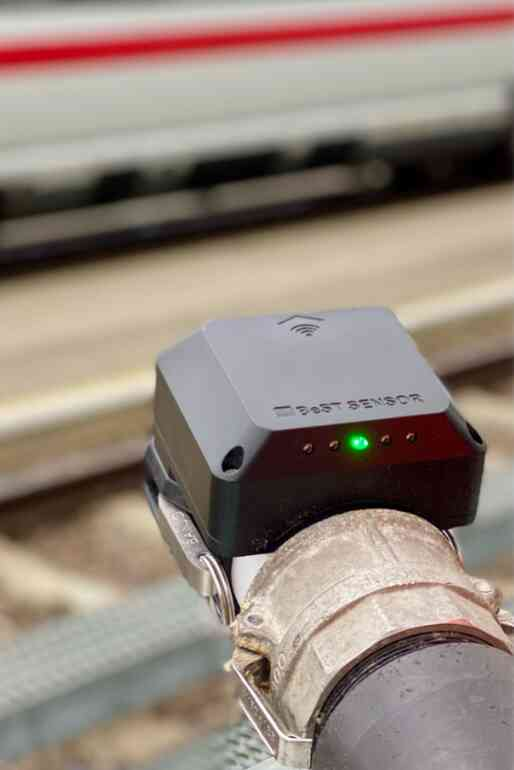
\includegraphics[width=0.45\textwidth]{images/jrov2201_housing.jpg}
      \end{figure}
    \end{column}
  \end{columns}
\end{frame}
%%%%%%%%%%%%%%%%%%%%%%%%%%%%%%%%%%%%%%%%%%%%%%%%%%%%%%%%%%%%%%%%%%%%%%%%%%%%%%%
\begin{frame}[fragile]{Workshop Goals}
  \begin{columns}[]
    \begin{column}{0.6\textwidth}
      \begin{itemize}
        \item Combine theory with hands-on practice
        \item Introduction to Zephyr RTOS
        \item Setting up the SDK
          \begin{itemize}
            \item On a Local Machine
            \item GitHub Codespaces
          \end{itemize}
        \item Exploring some of Zephyr's key features
        \item Hands-on Sessions
          \begin{enumerate}
            \item Development environment setup
            \item Build and run samples
            \item Build Zephyr applications for different boards
            \item Extend an application
          \end{enumerate}
      \end{itemize}
    \end{column}
    \begin{column}{0.4\textwidth}
    \end{column}
  \end{columns}
\end{frame}
%%%%%%%%%%%%%%%%%%%%%%%%%%%%%%%%%%%%%%%%%%%%%%%%%%%%%%%%%%%%%%%%%%%%%%%%%%%%%%%
\begin{frame}[fragile]{Workshop Goals - Audience}
  \begin{columns}[]
    \begin{column}{0.6\textwidth}
      \begin{itemize}
        \item What are your goals for the Workshop?
        \item Have you used an RTOS before?
        \item Your experience with Zephyr?
      \end{itemize}
    \end{column}
    \begin{column}{0.4\textwidth}
    \end{column}
  \end{columns}
\end{frame}
%%%%%%%%%%%%%%%%%%%%%%%%%%%%%%%%%%%%%%%%%%%%%%%%%%%%%%%%%%%%%%%%%%%%%%%%%%%%%%%
\begin{frame}[fragile]{Introduction to the Zephyr Project}
  \begin{columns}
    \begin{column}{0.6\textwidth}
      \begin{itemize}
        \item More than an RTOS, IoT ecosystm
        \item Microcontrollers, wireless SoCs to multicore SoCs
        \item Alternative to vendor SDKs
        \item Industry increasingly adopts Zephyr
        \item Set to be primary IoT ecosystem, if resource constraints do not allow to run Linux
      \end{itemize}
    \end{column}
    \begin{column}{0.4\textwidth}
      \begin{figure}
        \includegraphics[width=0.8\textwidth]{images/zephyr_logo.png}
        \caption*{The Zephyr Project logo}
      \end{figure}
    \end{column}
  \end{columns}
\end{frame}
%%%%%%%%%%%%%%%%%%%%%%%%%%%%%%%%%%%%%%%%%%%%%%%%%%%%%%%%%%%%%%%%%%%%%%%%%%%%%%%
\begin{frame}[fragile]{Introduction to the Zephyr Project}
  \begin{figure}
    \includegraphics[width=0.55\textwidth]{images/system-architecture.png}
    \caption*{\href{https://docs.zephyrproject.org/latest/security/security-overview.html}{docs.zephyrproject.org/latest/security/security-overview.html}}
  \end{figure}
\end{frame}
%%%%%%%%%%%%%%%%%%%%%%%%%%%%%%%%%%%%%%%%%%%%%%%%%%%%%%%%%%%%%%%%%%%%%%%%%%%%%%%
\begin{frame}[fragile]{Open Source and Vendor-Neutral Governance}
  \begin{columns}
    \begin{column}{0.6\textwidth}
      \begin{itemize}
        \item Governed by the Linux Foundation
        \item Vendor-neutrality: fairness and interoperability
        \item Technical Steering Committee (TSC) and Working Groups (WG) make technical decisions
        \item Security and tooling (e.g. SBOM) as integral part
        \item Safety certification ongoing
      \end{itemize}
    \end{column}
    \begin{column}{0.4\textwidth}
      \begin{figure}
        \includesvg[width=0.7\textwidth]{images/lf-stacked-color}
        \caption*{The Linux Foundation logo}
      \end{figure}
    \end{column}
  \end{columns}
\end{frame}
%%%%%%%%%%%%%%%%%%%%%%%%%%%%%%%%%%%%%%%%%%%%%%%%%%%%%%%%%%%%%%%%%%%%%%%%%%%%%%%
\begin{frame}[fragile]{Zephyr for products}

  \begin{block}{Examples}
    \begin{itemize}
       \item Overview: {\scriptsize \url{https://www.zephyrproject.org/products-running-zephyr/}}
       \item Wildlife Tracking and Protection (OpenCollar)
       \item Wind Turbines (Vestas)
       \item Irrigation (Gardena)
       \item Hearing Aid (Oticon)
       \item Wastewater Pump Monitoring (BeST Berliner Sensortechnik, German Railways - DB)
    \end{itemize}

  \end{block}
\end{frame}
%%%%%%%%%%%%%%%%%%%%%%%%%%%%%%%%%%%%%%%%%%%%%%%%%%%%%%%%%%%%%%%%%%%%%%%%%%%%%%%
\section{Development Setup}
% Explain General Development Setup
% Introduce Github code Spaces
%%%%%%%%%%%%%%%%%%%%%%%%%%%%%%%%%%%%%%%%%%%%%%%%%%%%%%%%%%%%%%%%%%%%%%%%%%%%%%%
\begin{frame}[fragile]{Getting Started Guide}
  \begin{figure}
    \includegraphics[width=\textwidth]{images/zephyr_getting_started.png}
    \caption*{\scriptsize\href{https://docs.zephyrproject.org/latest/getting_started/index.html}{https://docs.zephyrproject.org/latest/getting\_started/index.html}}
  \end{figure}
\end{frame}
%%%%%%%%%%%%%%%%%%%%%%%%%%%%%%%%%%%%%%%%%%%%%%%%%%%%%%%%%%%%%%%%%%%%%%%%%%%%%%%
\begin{frame}[fragile]{Setting up a Local Development Environment}
Linux, macOS and Windows \footnotemark  are supported!

Components:
  \begin{description}
    \item [Packages] git, cmake, python ..
    \item [Zephyr SDK] Toolchains for different architectures (compiler assembler..)
    \item [Python Tools] west, Install packages from requirements.txt in a virtual environment
    \item [IDE] Text editor, IDE (e.g. VSCode)
    \item [Repositories] Zephyr, modules via west
  \end{description}
	\footnotetext{Windows is supported, but will complicate development for
	Embedded Systems (e.g. no onboard package manager, often inconsistent
	Python environment setups).}
\end{frame}
%%%%%%%%%%%%%%%%%%%%%%%%%%%%%%%%%%%%%%%%%%%%%%%%%%%%%%%%%%%%%%%%%%%%%%%%%%%%%%%
\begin{frame}[fragile]{Testing the Local Development Environment}
  \begin{columns}
    \begin{column}{0.6\textwidth}
%-----------------------------------------
    Build and flash the application with \texttt{west}
    \begin{minted}[
      linenos,
      numbersep=15pt,
      framesep=2mm,
      bgcolor=lightgray!20,
      baselinestretch=1.1,
      fontsize=\scriptsize,
      firstnumber=1,
      stepnumber=5,
    ]{shell}
cd ~/zephyrproject/zephyr
west build -b reel_board samples/basic/blinky -p
west flash
    \end{minted}
    \begin{minted}[
      linenos,
      numbersep=15pt,
      framesep=2mm,
      bgcolor=lightgray!20,
      baselinestretch=1.1,
      fontsize=\scriptsize,
      firstnumber=1,
      stepnumber=5,
    ]{shell}
cd ~/zephyrproject/zephyr
west build -b native_sim samples/hello_world/ -p
west build -t run


*** Booting Zephyr OS build v4.1.0 ***
Hello World! native_sim/native
    \end{minted}
%-----------------------------------------
    \end{column}
    \begin{column}{0.4\textwidth}
      \begin{figure}
        \includegraphics[width=0.8\textwidth]{images/zephyr_blinky.png}
        \caption*{reel board with blinking LED}
      \end{figure}
    \end{column}
  \end{columns}
\end{frame}
%%%%%%%%%%%%%%%%%%%%%%%%%%%%%%%%%%%%%%%%%%%%%%%%%%%%%%%%%%%%%%%%%%%%%%%%%%%%%%%
\begin{frame}[fragile]{Starting a Cloud Development Environment}
  \begin{columns}
    \begin{column}{0.6\textwidth}
%-----------------------------------------
    GitHub Codespaces \footnotemark
    \begin{itemize}
      \item Cloud hosted development environment based on devcontainers
      \item Visual Studio Code integration
      \item Runs on Microsoft Azure cloud
      \item Configuration individual for each repository
    \end{itemize}
%-----------------------------------------
    \end{column}
    \begin{column}{0.4\textwidth}
      \begin{figure}
        \includegraphics[width=1.1\textwidth]{images/codespaces_setting_up.png}
        \caption*{Codespaces starting..}
      \end{figure}
    \end{column}
  \end{columns}
  \footnotetext{Open Source Alternatives: Gitpod, Eclipse Theia and many more}
\end{frame}
%%%%%%%%%%%%%%%%%%%%%%%%%%%%%%%%%%%%%%%%%%%%%%%%%%%%%%%%%%%%%%%%%%%%%%%%%%%%%%%
\begin{frame}[fragile]{Active Instance of GitHub Codespace}
  \begin{columns}
    \begin{column}{0.4\textwidth}
      \begin{figure}
        \includegraphics[width=\textwidth]{images/codespaces_how_to_start.png}
        \caption{Create a new Codespace}
      \end{figure}
      \begin{figure}
        \includegraphics[width=0.7\textwidth]{images/codespaces_setting_up.png}
        \caption{Codespaces starting..}
      \end{figure}
    \end{column}
    \begin{column}{0.6\textwidth}
      \begin{figure}
        \includegraphics[width=\textwidth]{images/codespaces_open.png}
        \caption{Codespaces in a Browser Window}
      \end{figure}
    \end{column}
  \end{columns}
\end{frame}
%%%%%%%%%%%%%%%%%%%%%%%%%%%%%%%%%%%%%%%%%%%%%%%%%%%%%%%%%%%%%%%%%%%%%%%%%%%%%%%
\begin{frame}[fragile]{Recommendations from my Experience}
Virtual Machines in combination with embedded hw can bring their own problems.

Prioritize a local environment over a cloud environment
  \begin{itemize}
    \item Hardware is better accessible
    \item Better integration of your own tools
  \end{itemize}

        Check vendor tools that can enhance your Zephyr Dev Environment
\end{frame}
%%%%%%%%%%%%%%%%%%%%%%%%%%%%%%%%%%%%%%%%%%%%%%%%%%%%%%%%%%%%%%%%%%%%%%%%%%%%%%%
\subsection{Hands-on 1}
\begin{frame}[fragile]{But for Showcasing, Codespaces is great! - Hands-on 1}
  \begin{columns}
    \begin{column}{0.6\textwidth}
            Start your own Codespaces Instance now! \footnotemark

      \href{https://github.com/jonas-rem/zephyr-workshop}{github.com/jonas-rem/zephyr-workshop}

      Setup will take a few minutes..

      Test your setup with the Hello World example:
      \begin{itemize}
        \item \scriptsize west build -b native\_sim zephyr/samples/hello\_world -p
        \item \scriptsize west build -t run
      \end{itemize}
    \end{column}
    \begin{column}{0.4\textwidth}
      \begin{figure}
        \includegraphics[width=1.1\textwidth]{images/codespaces_setting_up_class.png}
        \caption*{Setup new Instance}
      \end{figure}
    \end{column}
  \end{columns}
        \footnotetext{\textbf{Recommendation:} Use a 4-core setup instead of
                         the 2-core default.}
        \footnotetext{\textbf{Note:} You should have 120 core-hours per month free.}
\end{frame}
%%%%%%%%%%%%%%%%%%%%%%%%%%%%%%%%%%%%%%%%%%%%%%%%%%%%%%%%%%%%%%%%%%%%%%%%%%%%%%%
\section{Workspace Application and Hardware Abstraction}
% Out of Tree Build
% Explain devicetree
% Conditional Compilation (Different Code for different Boards)
% Coding Session 3 - Test on reel board
%%%%%%%%%%%%%%%%%%%%%%%%%%%%%%%%%%%%%%%%%%%%%%%%%%%%%%%%%%%%%%%%%%%%%%%%%%%%%%%
\begin{frame}[fragile]{Workspace Application}
  \begin{columns}
    \begin{column}{0.6\textwidth}
%-----------------------------------------
      \textbf{Workspace application} or \textbf{Out of tree} build \footnotemark[1]

      Separate application from Zephyr repository
      \begin{itemize}
        \item Independent version control for app
        \item Different Licences for app?
        \item Maintain references to Zephyr, Modules.. in app repo
        \item Update Zephyr version independently from app
      \end{itemize}

      Examples at \footnotemark[2]
%-----------------------------------------
    \end{column}
    \begin{column}{0.4\textwidth}
        {\fontsize{7}{7}\selectfont
          \begin{verbatim}
zephyrproject
├── modules
│   └── hal
├── zephyr
│   ├── samples
│   ├── west.yml
└── zephyr-workshop
    ├── west.yml
    └── samples
        └── 01_hello_world
            ├── CMakeLists.txt
            ├── prj.conf
            ├── README.rst
            ├── sample.yaml
            └── src
       \end{verbatim}
        }
    \end{column}
  \end{columns}
        \footnotetext[1]{\tiny\url{https://docs.zephyrproject.org/latest/develop/application/index.html}}
        \footnotetext[2]{\tiny\url{https://github.com/zephyrproject-rtos/example-application}}
        \footnotetext[2]{\tiny\url{https://github.com/jonas-rem/zephyr-workshop}}
\end{frame}
%%%%%%%%%%%%%%%%%%%%%%%%%%%%%%%%%%%%%%%%%%%%%%%%%%%%%%%%%%%%%%%%%%%%%%%%%%%%%%%
\begin{frame}[fragile]{Enabled by \texttt{west} and Manifest files}
  Manifests references repositories and modules \footnotemark[1]

  \begin{listing}[H]
    \begin{minted}[
      linenos,
      numbersep=15pt,
      framesep=2mm,
      bgcolor=lightgray!20,
      baselinestretch=1.1,
      fontsize=\scriptsize,
      firstnumber=1,
      stepnumber=5,
    ]{yaml}
manifest:
  remotes:
    - name: zephyrproject-rtos
      url-base: https://github.com/zephyrproject-rtos

  projects:
    - name: zephyr
      remote: zephyrproject-rtos
      revision: v3.6.0
      import:
        name-allowlist:
          - cmsis
          - hal_nordic
          - hal_nxp
          - [..]
    \end{minted}
    \caption{\scriptsize{\texttt{west.yaml} Manifest file in the zephyr-workshop repository}}
  \end{listing}
  \footnotetext[1]{\tiny\url{https://docs.zephyrproject.org/latest/develop/west/manifest.html}}
\end{frame}
%%%%%%%%%%%%%%%%%%%%%%%%%%%%%%%%%%%%%%%%%%%%%%%%%%%%%%%%%%%%%%%%%%%%%%%%%%%%%%%
\begin{frame}[fragile]{Understanding and Using \texttt{west}}
  \begin{columns}
    \begin{column}{0.6\textwidth}
      \texttt{west} repository management tool, developed by the Zephyr community
      \begin{itemize}
        \item Inspired by Google's Repo tool and git submodules
        \item Cloning Zephyr repo, dependencies, modules
        \item Keeping project repositories synchronized
        \item In addition building, flashing, and debugging support
      \end{itemize}

    \end{column}
    \begin{column}{0.4\textwidth}
        {\fontsize{6}{6}\selectfont
  \begin{listing}[H]
    \begin{minted}[
      framesep=2mm,
      bgcolor=lightgray!20,
      baselinestretch=1.1,
      fontsize=\tiny,
    ]{shell}
# Navigate to the project root
$ cd zephyrproject

# Update all repositories
$ west update

=== updating zephyr (zephyr):
HEAD is now at 468eb56cf24 [..]
=== updating cmsis (modules/hal/cmsis):
HEAD is now at 4b96cbb [..]
=== updating hal_atmel (modules/hal/atmel):
HEAD is now at aad79bf [..]
    \end{minted}
  \end{listing}
        }
    \end{column}
  \end{columns}
\end{frame}
%%%%%%%%%%%%%%%%%%%%%%%%%%%%%%%%%%%%%%%%%%%%%%%%%%%%%%%%%%%%%%%%%%%%%%%%%%%%%%%
\begin{frame}[fragile]{Application Structure - Use Case I}
  \begin{columns}
    \begin{column}{0.6\textwidth}
      \begin{description}
         \item[Who] User creates one application for testing
         \item[What] One variant of an application
         \item[Solution] Make changes inside the Zephyr tree for simplicity \footnotemark
      \end{description}
    \end{column}
    \begin{column}{0.4\textwidth}
      \begin{figure}
        \hspace*{1.5cm}
        \includesvg[width=0.8\textwidth]{images/application_topologies_1.svg}
      \end{figure}
    \end{column}
  \end{columns}
  \footnotetext{Not recommended production, use an out-of-tree build instead. This makes it easier to upgrade to more recent Zephyr versions.}
\end{frame}
%%%%%%%%%%%%%%%%%%%%%%%%%%%%%%%%%%%%%%%%%%%%%%%%%%%%%%%%%%%%%%%%%%%%%%%%%%%%%%%
\begin{frame}[fragile]{Application Structure - Use Case II}
  \begin{columns}
    \begin{column}{0.6\textwidth}
      \begin{description}
         \item[Who] One company developing one product
         \item [What] Two variants of the product
         \item Different sensors, pin assignments, but similar application
         \item[Solution] Devicetrees for each variant
         \item board\_a.dts: {\scriptsize\texttt{west build -b board\_a app}}
         \item board\_b.dts: {\scriptsize\texttt{west build -b board\_b app}}
      \end{description}
    \end{column}
    \begin{column}{0.4\textwidth}
      \begin{figure}
        \hspace*{0.4cm}
        \includesvg[width=\textwidth]{images/application_topologies_2.svg}
      \end{figure}
    \end{column}
  \end{columns}
\end{frame}
%%%%%%%%%%%%%%%%%%%%%%%%%%%%%%%%%%%%%%%%%%%%%%%%%%%%%%%%%%%%%%%%%%%%%%%%%%%%%%%
\begin{frame}[fragile]{Application Structure - Use Case III}
  \begin{columns}
    \begin{column}{0.6\textwidth}
      \begin{description}
         \item[Who] One company developing multiple products
         \item[What] Different applications
         \item[Solution] Seperate applications
         \item Use same Zephyr version for all applications if you can
      \end{description}
    \end{column}
    \begin{column}{0.4\textwidth}
      \begin{figure}
        \hspace*{-0.5cm}
        \includesvg[width=1.17\textwidth]{images/application_topologies_3.svg}
      \end{figure}
    \end{column}
  \end{columns}
\end{frame}
%%%%%%%%%%%%%%%%%%%%%%%%%%%%%%%%%%%%%%%%%%%%%%%%%%%%%%%%%%%%%%%%%%%%%%%%%%%%%%%
\begin{frame}[fragile]{Application Structure - Use Case IV}
  \begin{columns}
    \begin{column}{0.6\textwidth}
      \begin{description}
         \item[Who] Service provider developing different products for multiple companies
         \item[What] Development states and lifecycle for products differ
         \item[Solution] Individual manifest files for each product
         \item Create your own modules, share code inbetween projects
         \item Quickly setup and reference projecs with west
      \end{description}
    \end{column}
    \begin{column}{0.4\textwidth}
      \begin{figure}
        \hspace*{-0.5cm}
        \includesvg[width=1.17\textwidth]{images/application_topologies_4.svg}
      \end{figure}
    \end{column}
  \end{columns}
\end{frame}
%%%%%%%%%%%%%%%%%%%%%%%%%%%%%%%%%%%%%%%%%%%%%%%%%%%%%%%%%%%%%%%%%%%%%%%%%%%%%%%
\begin{frame}[fragile]{Zephyr Hardware Abstraction}
  \begin{columns}
    \begin{column}{0.6\textwidth}
%-----------------------------------------
      \begin{description}
          \item [Vendor HALs] Hardware abstraction available from vendors.
                  Abstracted via Zephyr APIs and drivers
          \item [Devicetree] Decouples the application from the hardware
          \item [Architecture] ARM, RISC-V, x86, ARC, NIOS II, Tensilica, Xtensa
          \item [Other] 600+ boards, 180+ sensors
      \end{description}
%-----------------------------------------
    \end{column}
    \begin{column}{0.4\textwidth}
      \begin{listing}[H]
        \begin{minted}[
          framesep=2mm,
          bgcolor=lightgray!20,
          baselinestretch=1.1,
          fontsize=\tiny,
        ]{console}
zephyrproject/zephyr:~$ ls arch/
arc    CMakeLists.txt  mips   riscv  xtensa
arm    common          nios2  sparc
arm64  Kconfig         posix  x86

zephyrproject:~$ ls modules/hal/
altera        espressif   nordic      silabs
ambiq         ethos_u     nuvoton     st
atmel         gigadevice  nxp         stm32
cirrus-logic  infineon    openisa     telink
[..]

zephyrproject/zephyr:~$ ls boards/
96boards               firefly       qemu
actinius               gd            rak
adafruit               google        raspberrypi
digilent               nordic        u-blox
enjoydigital           phytec        wemos
espressif              pine64        wiznet
[..]

zephyrproject/zephyr:~$ ls drivers/sensor/
adxl367                max30101
hs300x                 sht4x
ina3221                tcs3400
isl29035               th02
lps22hb                vl53l1x
[..]
        \end{minted}
      \end{listing}
    \end{column}
  \end{columns}
\end{frame}
%%%%%%%%%%%%%%%%%%%%%%%%%%%%%%%%%%%%%%%%%%%%%%%%%%%%%%%%%%%%%%%%%%%%%%%%%%%%%%%
\begin{frame}[fragile]{Zephyr Hardware Abstraction - devicetree}
  \begin{columns}
    \begin{column}{0.6\textwidth}
      Describes the available hardware
        \begin{itemize}
          \item Proven concept used in the Linux kernel
          \item Single source for hardware information
          \item Drivers and source are hardware independent
        \end{itemize}

      In Zephyr: C header generation at compile time
    \end{column}
    \begin{column}{0.4\textwidth}
      \begin{figure}
        \hspace*{-0.5cm}
        \includesvg[width=0.6\textwidth]{images/devicetree-logo.svg}
              \caption*{devicetree Logo\footnotemark}
      \end{figure}
      \footnotetext{\tiny\url{https://www.devicetree.org/}}
    \end{column}
  \end{columns}
\end{frame}
%%%%%%%%%%%%%%%%%%%%%%%%%%%%%%%%%%%%%%%%%%%%%%%%%%%%%%%%%%%%%%%%%%%%%%%%%%%%%%%
\begin{frame}[fragile]{Zephyr Hardware Abstraction - devicetree}
  \begin{listing}[H]
    \begin{minted}[
      framesep=2mm,
      bgcolor=lightgray!20,
      baselinestretch=1.1,
      fontsize=\tiny,
    ]{dts}
arduino_i2c: &i2c0 {
        compatible = "nordic,nrf-twim";
        status = "okay";
        clock-frequency = <I2C_BITRATE_FAST>;

        pinctrl-0 = <&i2c0_default>;
        pinctrl-1 = <&i2c0_sleep>;
        pinctrl-names = "default", "sleep";
        mma8642fc: mma8652fc@1d {
                compatible = "nxp,fxos8700","nxp,mma8652fc";
                reg = <0x1d>;
                int1-gpios = <&gpio0 24 GPIO_ACTIVE_LOW>;
                int2-gpios = <&gpio0 25 GPIO_ACTIVE_LOW>;
        };

        ti_hdc@43 {
                compatible = "ti,hdc","ti,hdc1010";
                reg = <0x43>;
                drdy-gpios = <&gpio0 22 (GPIO_ACTIVE_LOW | GPIO_PULL_UP)>;
        };

        apds9960@39 {
                compatible = "avago,apds9960";
                reg = <0x39>;
                int-gpios = <&gpio0 23 (GPIO_ACTIVE_LOW | GPIO_PULL_UP)>;
        };
};
    \end{minted}
          \caption{\scriptsize{devicetree node for the reel board: \texttt{boards/phytec/reel\_board/dts/reel\_board.dtsi}}}
  \end{listing}
\end{frame}
%%%%%%%%%%%%%%%%%%%%%%%%%%%%%%%%%%%%%%%%%%%%%%%%%%%%%%%%%%%%%%%%%%%%%%%%%%%%%%%
\subsection{Hands-on 2}
\begin{frame}[fragile]{Let's build Zephyr for the reel board! - Hands-on 2}
  \begin{columns}
    \begin{column}{0.6\textwidth}
       Build the \texttt{blinky} sample:
       \begin{itemize}
               \item \tiny\texttt{west build -b reel\_board ../zephyr/samples/basic/blinky -p}
       \end{itemize}

       Flash via Drag and Drop:
       \begin{itemize}
         \item \scriptsize{Download the binary from your Codespace at:} \scriptsize\texttt{build/zephyr/zephyr.hex}
         \item Drag and drop the hex file to the mounted reel board mass storage device on your machine
       \end{itemize}

       Flash via native setup:
       \begin{itemize}
         \item \scriptsize\texttt{west flash}
       \end{itemize}

       Attach to the serial console with e.g.:
       \begin{itemize}
         \item \scriptsize\texttt{minicom -D /dev/ttyACM0 -b 115200}
       \end{itemize}

    \end{column}
    \begin{column}{0.4\textwidth}
      \begin{figure}
        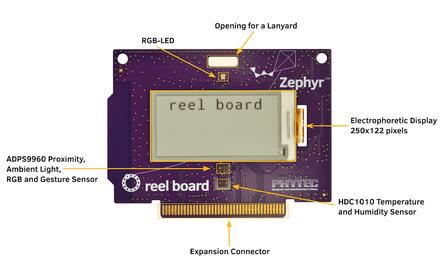
\includegraphics[width=.9\textwidth]{images/reel_board.jpg}
      \end{figure}
      \begin{figure}
        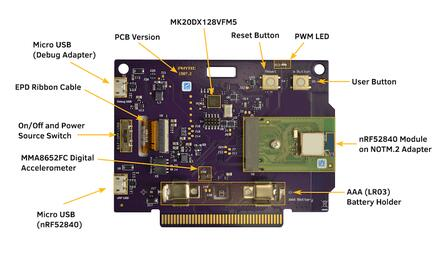
\includegraphics[width=.9\textwidth]{images/reel_board_descr_back.jpg}
      \end{figure}
    \end{column}
  \end{columns}
\end{frame}
%%%%%%%%%%%%%%%%%%%%%%%%%%%%%%%%%%%%%%%%%%%%%%%%%%%%%%%%%%%%%%%%%%%%%%%%%%%%%%%
%%%%%%%%%%%%%%%%%%%%%%%%%%%%%%%%%%%%%%%%%%%%%%%%%%%%%%%%%%%%%%%%%%%%%%%%%%%%%%%
\section{Code Examples and Subsystems}
% Explain simple code examples
% Showcase the Codespaces environment to everyone
% Let the audience try out the Codespaces environment, give a coding task
% -> Timer and workqueue example
%%%%%%%%%%%%%%%%%%%%%%%%%%%%%%%%%%%%%%%%%%%%%%%%%%%%%%%%%%%%%%%%%%%%%%%%%%%%%%%
\begin{frame}[fragile]{Samples in Zephyr}

  \begin{block}{Samples}
    \begin{itemize}
      \item Zephyr provides a wide range of samples
      \item Samples are located in \texttt{zephyr/samples/}
      \item Isolated functionality or feature
    \end{itemize}
  \end{block}
  \begin{block}{Tests}
    \begin{itemize}
      \item Tests are located in \texttt{zephyr/tests/}
      \item Isolated test cases for a feature or hardware
      \item Useful to test e.g. a device driver
    \end{itemize}
  \end{block}
  \begin{block}{Applications}
    \begin{itemize}
      \item Application Example: {\scriptsize \url{https://github.com/zephyrproject-rtos/example-application}}
      \item ZSWatch - Open Source Smart Watch: {\scriptsize \url{https://github.com/jakkra/ZSWatch}}
    \end{itemize}
  \end{block}
\end{frame}
%%%%%%%%%%%%%%%%%%%%%%%%%%%%%%%%%%%%%%%%%%%%%%%%%%%%%%%%%%%%%%%%%%%%%%%%%%%%%%%
\begin{frame}[fragile]{01\_hello\_world}
  \begin{columns}
    \begin{column}{0.6\textwidth}
%-----------------------------------------
      \begin{description}
        \item [Description] Simple Hello World program \footnotemark
        \item [Learn] Test setup
        \item Structure of a Zephyr application
      \end{description}
      \begin{block}{Build and run}
      \begin{itemize}
        \item \scriptsize west build -b qemu\_cortex\_m0 samples/01\_hello\_world -p
        \item \scriptsize west build -t run
      \end{itemize}
      \end{block}
%-----------------------------------------
    \end{column}
    \begin{column}{0.4\textwidth}
        {\fontsize{7}{7}\selectfont
          \begin{verbatim}
samples/01_hello_world/
├── CMakeLists.txt
├── prj.conf
├── README.rst
├── sample.yaml
├── 01_hello_world
└── src
    └── main.c
          \end{verbatim}
        }
    \end{column}
  \end{columns}
  \footnotetext{Equivalent in the Zephyr main Repository: zephyr/samples/hello\_world.}
\end{frame}
%%%%%%%%%%%%%%%%%%%%%%%%%%%%%%%%%%%%%%%%%%%%%%%%%%%%%%%%%%%%%%%%%%%%%%%%%%%%%%%
\begin{frame}[fragile]{01\_hello\_world Configuring the Build System}
\inputmintedpath{cmake}{../samples/01_hello_world/CMakeLists.txt}
\end{frame}
%%%%%%%%%%%%%%%%%%%%%%%%%%%%%%%%%%%%%%%%%%%%%%%%%%%%%%%%%%%%%%%%%%%%%%%%%%%%%%%
\begin{frame}[fragile]{01\_hello\_world Application Source Code}
\inputmintedpath{c}{../samples/01_hello_world/src/main.c}
\end{frame}
%%%%%%%%%%%%%%%%%%%%%%%%%%%%%%%%%%%%%%%%%%%%%%%%%%%%%%%%%%%%%%%%%%%%%%%%%%%%%%
\begin{frame}[fragile]{01\_hello\_world Application Build Output}
  \begin{listing}[H]
    \begin{minted}[
      linenos,
      numbersep=15pt,
      framesep=2mm,
      bgcolor=lightgray!20,
      baselinestretch=1.1,
      fontsize=\scriptsize,
      firstnumber=1,
      stepnumber=5,
    ]{shell}
west build -b qemu_cortex_m0 samples/01_hello_world/ -p
-- Found host-tools: zephyr 0.17.0 (/home/jonas/zephyr-sdk-0.17.0)
-- Found toolchain: zephyr 0.17.0 (/home/jonas/zephyr-sdk-0.17.0)
[..]
Parsing /home/jonas/git/zephyrproject/zephyr/Kconfig
-- The C compiler identification is GNU 12.2.0
-- The CXX compiler identification is GNU 12.2.0
-- The ASM compiler identification is GNU
-- Found assembler: /home/jonas/zephyr-sdk-0.17.0/arm-zephyr-eabi/bin/arm-zephyr-eabi-gcc
-- Configuring done (3.0s)
-- Generating done (0.1s)
-- Build files have been written to: /home/jonas/git/zephyrproject/zephyr-workshop/build
-- west build: building application
[1/117] Preparing syscall dependency handling

[2/117] Generating include/generated/zephyr/version.h
-- Zephyr version: 4.1.0 (/home/jonas/git/zephyrproject/zephyr), build: v4.1.0
[117/117] Linking C executable zephyr/zephyr.elf
Memory region         Used Size  Region Size  %age Used
           FLASH:        8094 B       256 KB      3.09%
             RAM:          4 KB        64 KB      6.25%
        IDT_LIST:          0 GB        32 KB      0.00%
    \end{minted}
  \caption{\scriptsize{Console Output}}
  \end{listing}
\end{frame}
%%%%%%%%%%%%%%%%%%%%%%%%%%%%%%%%%%%%%%%%%%%%%%%%%%%%%%%%%%%%%%%%%%%%%%%%%%%%%%%
\begin{frame}[fragile]{01\_hello\_world Build Artifacts}
  \begin{columns}
    \begin{column}{0.6\textwidth}
%-----------------------------------------
      \begin{description}
        \item [Build Location] \texttt{build/}
        \item [Executable Location] \texttt{build/zephyr/}
        \item [Artifacts]
          \begin{itemize}
            \item \texttt{zephyr.elf|hex|bin}
            \item \texttt{zephyr.map}
            \item \texttt{autoconf.h} (Kconfig options)
            \item \texttt{autoconf.h} (Generated devicetree header)
            \item \texttt{Kconfig.dts} (devicetree conf)
          \end{itemize}
      \end{description}
%-----------------------------------------
    \end{column}
    \begin{column}{0.4\textwidth}
        {\fontsize{7}{7}\selectfont
          \begin{verbatim}
build/
├── app
│   └── libapp.a
├── Kconfig
│   └── Kconfig.dts
└── zephyr
    ├── include
    │   └── generated
    │      └── zephyr
    │         ├── autoconf.h
    │         ├── devicetree_generated.h
    ├── zephyr.dts
    ├── zephyr.elf|bin|hex
    ├── zephyr_final.map
          \end{verbatim}
        }
    \end{column}
  \end{columns}
\end{frame}
%%%%%%%%%%%%%%%%%%%%%%%%%%%%%%%%%%%%%%%%%%%%%%%%%%%%%%%%%%%%%%%%%%%%%%%%%%%%%%%
\begin{frame}[fragile]{01\_hello\_world Sample - Console Output}
  \begin{listing}[H]
    \begin{minted}[
      linenos,
      numbersep=15pt,
      framesep=2mm,
      bgcolor=lightgray!20,
      baselinestretch=1.1,
      fontsize=\scriptsize,
      firstnumber=1,
      stepnumber=5,
    ]{shell}
*** Booting Zephyr OS build v4.1.0 ***
Hello World! qemu_cortex_m3/ti_lm3s6965
    \end{minted}
  \caption{\scriptsize{Console Output}}
  \end{listing}
\end{frame}
%%%%%%%%%%%%%%%%%%%%%%%%%%%%%%%%%%%%%%%%%%%%%%%%%%%%%%%%%%%%%%%%%%%%%%%%%%%%%%%
\begin{frame}[fragile]{02\_logging Sample}
  \begin{columns}
    \begin{column}{0.6\textwidth}
      \begin{description}
	\item [Description] Logging subsystem example\footnotemark
	\item [Logging] Log levels
	\item Set loglevel via Kconfig
	\item Different Logging backends, e.g. filesystem, BLE
	\item Log messages printed in own thread when system is idle
	\item [Sample] Demonstrates logging output
      \end{description}
    \end{column}
    \begin{column}{0.4\textwidth}
        {\fontsize{6}{6}\selectfont
  \begin{listing}[H]
    \begin{minted}[
      framesep=2mm,
      bgcolor=lightgray!20,
      baselinestretch=1.1,
      fontsize=\tiny,
    ]{Kconfig}
CONFIG_LOG=y
    \end{minted}
    \caption{\scriptsize{Excerpt from samples/02\_logging/prj.conf}}
  \end{listing}
  \begin{listing}[H]
    \begin{minted}[
      framesep=2mm,
      bgcolor=lightgray!20,
      baselinestretch=1.1,
      fontsize=\tiny,
    ]{c}
#include <zephyr/logging/log.h>

LOG_MODULE_REGISTER(hello_world, LOG_LEVEL_DBG);

int main(void)
{
	LOG_INF("info string");

	return 0;
}
    \end{minted}
  \caption{\scriptsize{Excerpt from samples/02\_logging/src/main.c}}
  \end{listing}
        }
    \end{column}
  \end{columns}
  \footnotetext{Equivalent in the Zephyr main Repository: zephyr/samples/subsys/logging/logger.}
\end{frame}
%%%%%%%%%%%%%%%%%%%%%%%%%%%%%%%%%%%%%%%%%%%%%%%%%%%%%%%%%%%%%%%%%%%%%%%%%%%%%%%
\begin{frame}[fragile]{02\_logging Sample - Console Output}
  \begin{listing}[H]
    \begin{minted}[
      linenos,
      numbersep=15pt,
      framesep=2mm,
      bgcolor=lightgray!20,
      baselinestretch=1.1,
      fontsize=\scriptsize,
      firstnumber=1,
      stepnumber=5,
    ]{shell}
*** Booting Zephyr OS build v4.1.0 ***
Hello World! qemu_cortex_m0
[00:00:00.001,691] <err> hello_world: error string
[00:00:00.001,843] <dbg> hello_world: main: debug string
[00:00:00.001,859] <inf> hello_world: info string
[00:00:00.001,874] <dbg> hello_world: main: int8_t 1, uint8_t 2
[00:00:00.001,887] <dbg> hello_world: main: int16_t 16, uint16_t 17
[00:00:00.001,899] <dbg> hello_world: main: int32_t 32, uint32_t 33
[00:00:00.001,921] <dbg> hello_world: main: int64_t 64, uint64_t 65
[00:00:00.001,956] <dbg> hello_world: main: char !
[00:00:00.002,383] <dbg> hello_world: main: s str static str c str
[00:00:00.002,567] <dbg> hello_world: main: d str dynamic str
[00:00:00.002,607] <dbg> hello_world: main: mixed str dynamic str --- dynamic str --- da --- da
[00:00:00.002,640] <dbg> hello_world: main: mixed c/s ! static str dynamic str static str !
[00:00:00.002,653] <dbg> hello_world: main: pointer 0x5c3e
[00:00:00.002,674] <dbg> hello_world: main: HeXdUmP!
                                      48 45 58 44 55 4d 50 21  20 23 40                |HEXDUMP!  #@

    \end{minted}
  \end{listing}
\end{frame}
%%%%%%%%%%%%%%%%%%%%%%%%%%%%%%%%%%%%%%%%%%%%%%%%%%%%%%%%%%%%%%%%%%%%%%%%%%%%%%%
\begin{frame}[fragile]{03\_workqueues Sample}
      \begin{description}
	\item [Description] Workqueue and Timer Example
	\item [Learn] Workqueue, Timers, Runtime Contexts (IRQ, Thread)
	\item Queue of work items
	\item Work items are executed in a thread context
	\item Timer is used to schedule work items
	\item System workqueue is enabled by default
	\item [Sample] Executes a function in different contexts
      \end{description}
\end{frame}
%%%%%%%%%%%%%%%%%%%%%%%%%%%%%%%%%%%%%%%%%%%%%%%%%%%%%%%%%%%%%%%%%%%%%%%%%%%%%%%
\begin{frame}[fragile]{03\_workqueues Sample - Console Output}
  \begin{listing}[H]
    \begin{minted}[
      linenos,
      numbersep=15pt,
      framesep=2mm,
      bgcolor=lightgray!20,
      baselinestretch=1.1,
      fontsize=\scriptsize,
      firstnumber=1,
      stepnumber=5,
    ]{shell}
 *** Booting Zephyr OS build v4.1.0 ***
Work Item Executed - runtime context:
 Thread Name: main
 Thread Priority: 0

Work Item Executed - runtime context:
 Thread Name: sysworkq
 Thread Priority: -1

Work Item Executed - runtime context:
 Thread Name: my_work_q_thread
 Thread Priority: 5

Timer Expired!!
Work Item Executed - runtime context:
 ISR Context!

Work Item Executed - runtime context:
 Thread Name: sysworkq
 Thread Priority: -1
    \end{minted}
  \end{listing}
\end{frame}
%%%%%%%%%%%%%%%%%%%%%%%%%%%%%%%%%%%%%%%%%%%%%%%%%%%%%%%%%%%%%%%%%%%%%%%%%%%%%%%
\begin{frame}[fragile]{04\_shell Sample}
  \begin{columns}
    \begin{column}{0.6\textwidth}
      \begin{description}
	\item [Description] Shell subsystem example\footnotemark
	\item [Shell] Command line interface
	\item Command history, completion, help
	\item Great for testing and debugging
	\item [Sample] Provides a basic shell
      \end{description}
    \end{column}
    \begin{column}{0.4\textwidth}
        {\fontsize{6}{6}\selectfont
  \begin{listing}[H]
    \begin{minted}[
      framesep=2mm,
      bgcolor=lightgray!20,
      baselinestretch=1.1,
      fontsize=\tiny,
    ]{Kconfig}
CONFIG_SHELL=y

# Optional features
CONFIG_THREAD_STACK_INFO=y
CONFIG_KERNEL_SHELL=y
CONFIG_THREAD_MONITOR=y
CONFIG_BOOT_BANNER=n
CONFIG_THREAD_NAME=y
CONFIG_DEVICE_SHELL=y
CONFIG_POSIX_CLOCK=y
CONFIG_DATE_SHELL=y
CONFIG_THREAD_RUNTIME_STATS=y
CONFIG_THREAD_RUNTIME_STATS_USE_TIMING_FUNCTIONS=y
CONFIG_STATS=y
CONFIG_STATS_SHELL=y
    \end{minted}
    \caption{\scriptsize{Excerpt from samples/04\_shell/prj.conf}}
  \end{listing}
        }
    \end{column}
  \end{columns}
  \footnotetext{Equivalent in the Zephyr main Repository: zephyr/samples/subsys/shell/shell\_module.}
\end{frame}
%%%%%%%%%%%%%%%%%%%%%%%%%%%%%%%%%%%%%%%%%%%%%%%%%%%%%%%%%%%%%%%%%%%%%%%%%%%%%%%
\begin{frame}[fragile]{04\_shell Sample - Console Output}
  \begin{listing}[H]
    \begin{minted}[
      linenos,
      numbersep=15pt,
      framesep=2mm,
      bgcolor=lightgray!20,
      baselinestretch=1.1,
      fontsize=\tiny,
      firstnumber=1,
      stepnumber=5,
    ]{shell}
uart:~$ 
  bypass              clear               date
  demo                device              devmem
  dynamic             help                history
  kernel              log                 log_test
  rem                 resize              retval
  section_cmd         shell               shell_uart_release
  stats               version
uart:~$ kernel thread list
Threads:
*0x20000720 shell_uart
	options: 0x0, priority: 14 timeout: 0
	state: queued, entry: 0x3ed9
	Total execution cycles: 22360 (0 %)
	stack size 2048, unused 932, usage 1116 / 2048 (54 %)

 0x20001288 sysworkq
	options: 0x1, priority: -1 timeout: 0
	state: pending, entry: 0x7169
	Total execution cycles: 163 (0 %)
	stack size 1024, unused 808, usage 216 / 1024 (21 %)

 0x20000218 logging
	options: 0x0, priority: 14 timeout: 0
	state: pending, entry: 0x1861
	Total execution cycles: 237 (0 %)
	stack size 768, unused 576, usage 192 / 768 (25 %)

 0x20000fd0 idle
	options: 0x1, priority: 15 timeout: 0
	state: , entry: 0xb6c1
	Total execution cycles: 47021886 (99 %)
    \end{minted}
  \end{listing}
\end{frame}
%%%%%%%%%%%%%%%%%%%%%%%%%%%%%%%%%%%%%%%%%%%%%%%%%%%%%%%%%%%%%%%%%%%%%%%%%%%%%%%
\begin{frame}[fragile]{05\_sensor Sample}
  \begin{columns}
    \begin{column}{0.6\textwidth}
      \begin{description}
	\item [Description] TI HDC1010: I2C Temperature and Humidity Sensor \footnotemark
	\item [Sensor] Temperature and Humidity e.g. on the reel board
	\item [Sample] Demonstrates Sensor API
      \end{description}
    \end{column}
    \begin{column}{0.4\textwidth}
        {\fontsize{5}{5}\selectfont
  \begin{listing}[H]
    \begin{minted}[
      framesep=2mm,
      bgcolor=lightgray!20,
      baselinestretch=1.1,
      fontsize=\tiny,
    ]{c}
sensor_sample_fetch(dev);
sensor_channel_get(dev, SENSOR_CHAN_AMBIENT_TEMP,
	           &temp);
sensor_channel_get(dev, SENSOR_CHAN_HUMIDITY,
	           &humidity);

/* print the result */
printk("Temp = %d.%06d C, RH = %d.%06d %%\n",
       temp.val1, temp.val2,
       humidity.val1, humidity.val2);
    \end{minted}
    \caption{\scriptsize{Excerpt from samples/05\_sensor/src/main.c}}
  \end{listing}
        }
    \end{column}
  \end{columns}
  \footnotetext{Equivalent in the Zephyr main Repository: zephyr/samples/sensor/ti\_hdc.}
\end{frame}
%%%%%%%%%%%%%%%%%%%%%%%%%%%%%%%%%%%%%%%%%%%%%%%%%%%%%%%%%%%%%%%%%%%%%%%%%%%%%%%
\begin{frame}[fragile]{05\_sensor Sample - Console Output}
  \begin{listing}[H]
    \begin{minted}[
      linenos,
      numbersep=15pt,
      framesep=2mm,
      bgcolor=lightgray!20,
      baselinestretch=1.1,
      fontsize=\tiny,
      firstnumber=1,
      stepnumber=5,
    ]{shell}
*** Booting Zephyr OS build v4.1.0 ***
Running on arm!
Dev 0x801c name ti_hdc@43 is ready!
Fetching...
Temp = 22.852966 C, RH = 38.793945 %
Fetching...
Temp = 22.842895 C, RH = 38.897705 %
Fetching...
    \end{minted}
  \end{listing}
\end{frame}
%%%%%%%%%%%%%%%%%%%%%%%%%%%%%%%%%%%%%%%%%%%%%%%%%%%%%%%%%%%%%%%%%%%%%%%%%%%%%%%
\begin{frame}[fragile]{06\_ble Sample}
  \begin{columns}
    \begin{column}{0.6\textwidth}
      \begin{description}
     \item
	\item [Description] BLE Peripheral device, temperature monitor \footnotemark
	\item [Sample] App to connect: nRF Connect for Mobile (Android, iOS)
      \end{description}
    \end{column}
    \begin{column}{0.4\textwidth}
        {\fontsize{6}{6}\selectfont
  \begin{listing}[H]
    \begin{minted}[
      framesep=2mm,
      bgcolor=lightgray!20,
      baselinestretch=1.1,
      fontsize=\tiny,
    ]{Kconfig}
CONFIG_BT=y
CONFIG_LOG=y
CONFIG_BT_SMP=y
CONFIG_BT_PERIPHERAL=y
CONFIG_BT_DIS=y
CONFIG_BT_DIS_PNP=n
CONFIG_BT_BAS=y
CONFIG_BT_DEVICE_NAME="Zephyr Health Thermometer"
CONFIG_BT_DEVICE_APPEARANCE=768
CONFIG_CBPRINTF_FP_SUPPORT=y
    \end{minted}
    \caption{\scriptsize{Excerpt from samples/06\_ble/prj.conf}}
  \end{listing}
        }
    \end{column}
  \end{columns}
  \footnotetext{Equivalent in the Zephyr main Repository: zephyr/samples/bluetooth/peripheral\_ht.}
\end{frame}
%%%%%%%%%%%%%%%%%%%%%%%%%%%%%%%%%%%%%%%%%%%%%%%%%%%%%%%%%%%%%%%%%%%%%%%%%%%%%%%
\begin{frame}[fragile]{06\_ble Sample - Console Output}
  \begin{listing}[H]
    \begin{minted}[
      linenos,
      numbersep=15pt,
      framesep=2mm,
      bgcolor=lightgray!20,
      baselinestretch=1.1,
      fontsize=\tiny,
      firstnumber=1,
      stepnumber=5,
    ]{shell}
*** Booting Zephyr OS build v4.1.0 ***
[00:00:00.380,645] <inf> bt_hci_core: HW Platform: Nordic Semiconductor (0x0002)
[00:00:00.380,676] <inf> bt_hci_core: HW Variant: nRF52x (0x0002)
[00:00:00.380,706] <inf> bt_hci_core: Firmware: Standard Bluetooth controller (0x00) Version 4.1 Build 0
[00:00:00.381,347] <inf> bt_hci_core: Identity: D0:6F:6B:78:0C:E8 (random)
[00:00:00.381,378] <inf> bt_hci_core: HCI: version 5.4 (0x0d) revision 0x0000, manufacturer 0x05f1
[00:00:00.381,408] <inf> bt_hci_core: LMP: version 5.4 (0x0d) subver 0xffff
Bluetooth initialized
temp device is 0x28b5c, name is temp@4000c000
Advertising successfully started
Connected
temperature is 24C
temperature is 23.75C
Indication success
Indication complete
Indication success
Indication complete
temperature is 23.75C
temperature is 23.75C
    \end{minted}
  \end{listing}
\end{frame}
%%%%%%%%%%%%%%%%%%%%%%%%%%%%%%%%%%%%%%%%%%%%%%%%%%%%%%%%%%%%%%%%%%%%%%%%%%%%%%%
\begin{frame}[fragile]{06\_ble Sample - Connect with a Smartphone}
  \begin{columns}
    \begin{column}{0.5\textwidth}
      \begin{figure}
        \includegraphics[width=0.4\textwidth]{images/nrf_connect_scan.png}
        \caption*{Scanning for BLE devices}
      \end{figure}
    \end{column}
    \begin{column}{0.5\textwidth}
      \begin{figure}
        \includegraphics[width=0.4\textwidth]{images/nrf_connect_ble_connected.png}
        \caption*{Connected with nRF Connect App}
      \end{figure}
    \end{column}
  \end{columns}
\end{frame}
%%%%%%%%%%%%%%%%%%%%%%%%%%%%%%%%%%%%%%%%%%%%%%%%%%%%%%%%%%%%%%%%%%%%%%%%%%%%%%%
\begin{frame}[fragile]{07\_display\_cfb Sample - Controle the passive Display}
  \begin{columns}
    \begin{column}{0.6\textwidth}
      \begin{description}
        \item [Description] Character Framebuffer Sample \footnotemark
        \item [Sample] Writes text to the display
      \end{description}
    \end{column}
    \begin{column}{0.4\textwidth}
      \begin{figure}
        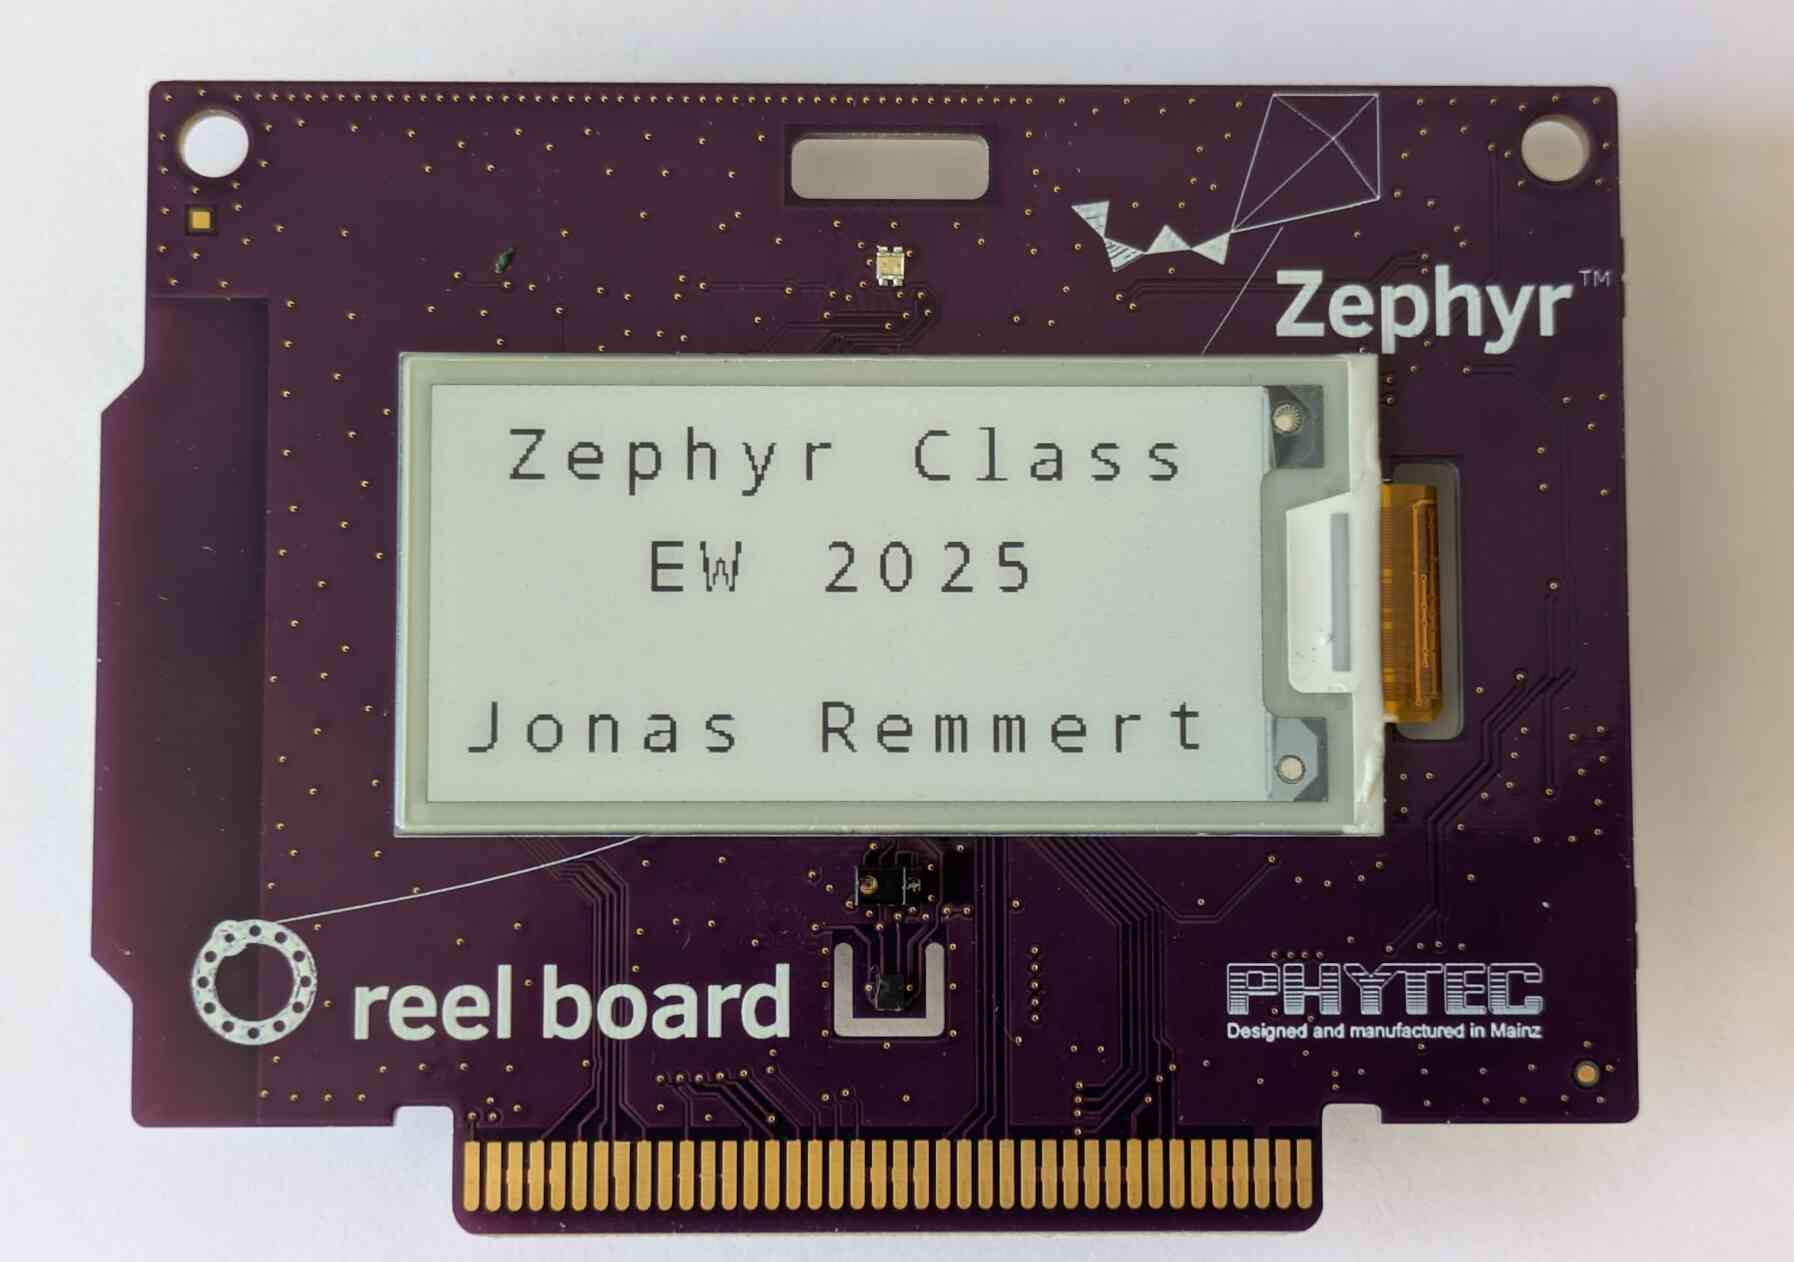
\includegraphics[width=\textwidth]{images/reel_board_passive_display.jpg}
        \caption*{Updated display on the reel board}
      \end{figure}
    \end{column}
  \end{columns}
  \footnotetext{Equivalent in the Zephyr main Repository: zephyr/samples/subsys/display/cfb.}
\end{frame}
%%%%%%%%%%%%%%%%%%%%%%%%%%%%%%%%%%%%%%%%%%%%%%%%%%%%%%%%%%%%%%%%%%%%%%%%%%%%%%%
\subsection{Hands-on 3}
\begin{frame}[fragile]{Test the Samples - Hands-on 3}
  \begin{columns}
    \begin{column}{0.6\textwidth}
      Build and run the samples\footnotemark:
      \begin{itemize}
        \item \scriptsize west build -b qemu\_cortex\_m0 samples/02\_logging -p
        \item \scriptsize west build -t run
	\item \scriptsize \texttt{or}
        \item \scriptsize west build -b reel\_board@2 samples/02\_logging -p
        \item \scriptsize west flash
      \end{itemize}
      Update the displayed name on the passive display
    \end{column}
    \begin{column}{0.4\textwidth}
        {\fontsize{7}{7}\selectfont
          \begin{verbatim}
samples
├── 01_hello_world
├── 02_logging
├── 03_workqueues
├── 04_shell
├── 05_sensor
├── 06_ble
└── 07_display_cfb
        \end{verbatim}
      }
    \end{column}
  \end{columns}
  \footnotetext{\textbf{Note:} The sensor and ble samples require a board to run.}
>>>>>>> ece9698 (slides: adapt slides to demonstrate with reel board)
\end{frame}
\section{Application Development}
% zbus, IPC, Threads
% Work with modularization, utlize the build system
% Hands On Excersies 4 - Extend a sample application
%%%%%%%%%%%%%%%%%%%%%%%%%%%%%%%%%%%%%%%%%%%%%%%%%%%%%%%%%%%%%%%%%%%%%%%%%%%%%%%
\begin{frame}[fragile]{IPC Mechanisms and Zephyr bus (Zbus)}
  \begin{columns}
    \begin{column}{0.6\textwidth}
%-----------------------------------------
      Mutexes, Semaphores

      Conditional Variables, Message Queues

      Polling API to wait for any out of multiple conditions

    \begin{block}{Zbus}
      \begin{itemize}
        \item Comparable to D-Bus in Linux
        \item Many-to-many communication
        \item Simplifies thread synchronization
      \end{itemize}
    \end{block}
%-----------------------------------------
    \end{column}
    \begin{column}{0.4\textwidth}
      \begin{figure}
       \includesvg[width=\textwidth]{images/zbus_zephyr.svg}
        \caption*{Zbus overview\footnotemark}
      \end{figure}
    \end{column}
  \end{columns}
  \footnotetext{\tiny\url{https://docs.zephyrproject.org/latest/services/zbus/index.html}}
\end{frame}
%%%%%%%%%%%%%%%%%%%%%%%%%%%%%%%%%%%%%%%%%%%%%%%%%%%%%%%%%%%%%%%%%%%%%%%%%%%%%%%
\begin{frame}[fragile]{Example Application}
  \begin{columns}
    \begin{column}{0.6\textwidth}
%-----------------------------------------
    Button
    \begin{itemize}
      \item Switch between system states (active, sleep)
    \end{itemize}

    LED
    \begin{itemize}
      \item Indicate system state
      \item Run in own thread for smooth animations
    \end{itemize}
%-----------------------------------------
    \end{column}
    \begin{column}{0.4\textwidth}
      \begin{figure}
       \includesvg[width=0.9\textwidth]{images/zbus_application.svg}
        \caption*{Minimal modular application with zbus}
      \end{figure}
    \end{column}
  \end{columns}
\end{frame}
%%%%%%%%%%%%%%%%%%%%%%%%%%%%%%%%%%%%%%%%%%%%%%%%%%%%%%%%%%%%%%%%%%%%%%%%%%%%%%%
\begin{frame}[fragile]{Example Application - Modular Development}
  \begin{columns}
    \begin{column}{0.6\textwidth}
%-----------------------------------------
      \begin{description}
        \item [General] Code reuse, maintainability, readability
	\item [IPC] Communication e.g. via Zbus
	\item Context of each module can be controlled
	\item [Testing] Modules can be tested seperately
      \end{description}
%-----------------------------------------
    \end{column}
    \begin{column}{0.4\textwidth}
        {\fontsize{6}{6}\selectfont
          \begin{verbatim}
app/
├── CMakeLists.txt
├── Kconfig
├── prj.conf
└── src
    ├── common
    │   ├── CMakeLists.txt
    │   ├── message_channel.c
    │   └── message_channel.h
    ├── main.c
    └── modules
        ├── button
        │   ├── button.c
        │   ├── CMakeLists.txt
        │   └── Kconfig.button
        └── led
            ├── CMakeLists.txt
            ├── Kconfig.led
            └── led.c
          \end{verbatim}
        }
    \end{column}
  \end{columns}
\end{frame}
%%%%%%%%%%%%%%%%%%%%%%%%%%%%%%%%%%%%%%%%%%%%%%%%%%%%%%%%%%%%%%%%%%%%%%%%%%%%%%%
\begin{frame}[fragile]{Example Application - Testing}
  \begin{columns}
    \begin{column}{0.6\textwidth}
%-----------------------------------------
      Isolated testing of modules

      Add subsystems like shell, ztest for test cases

      Tests reference modules via CMake

      Interfaces inbetween modules abstracted via zbus
%-----------------------------------------
    \end{column}
    \begin{column}{0.4\textwidth}
        {\fontsize{6}{6}\selectfont
          \begin{verbatim}
test/
├── button
│   ├── CMakeLists.txt
│   ├── Kconfig
│   ├── prj.conf
│   ├── sample.yaml
│   └── src
│       └── main.c
└── led
    ├── CMakeLists.txt
    ├── Kconfig
    ├── prj.conf
    ├── sample.yaml
    └── src
        └── main.c
          \end{verbatim}
        }
    \end{column}
  \end{columns}
\end{frame}
%%%%%%%%%%%%%%%%%%%%%%%%%%%%%%%%%%%%%%%%%%%%%%%%%%%%%%%%%%%%%%%%%%%%%%%%%%%%%%%
\begin{frame}[fragile]{Example Application - Testing Modules}
  \begin{listing}[H]
    \begin{minted}[
      framesep=2mm,
      bgcolor=lightgray!20,
      baselinestretch=1.1,
      fontsize=\tiny,
    ]{cmake}
target_sources(app PRIVATE src/main.c)
add_subdirectory(../../app/src/common common)
add_subdirectory(../../app/src/modules/button button)
    \end{minted}
    \caption{\footnotesize{Excerpt from : \texttt{test/button/CMakeLists.txt}}}
  \end{listing}
  \begin{listing}[H]
    \begin{minted}[
      framesep=2mm,
      bgcolor=lightgray!20,
      baselinestretch=1.1,
      fontsize=\tiny,
    ]{c}
void button_test_msg_cb(const struct zbus_channel *chan)
{
	const enum sys_msg *msg_type;

	msg_type = zbus_chan_const_msg(chan);
	if (msg_type == SYS_BUTTON_PRESSED) {
		LOG_INF("Button pressed!");
	}
}

ZBUS_LISTENER_DEFINE(button_test, button_test_msg_cb);
ZBUS_CHAN_ADD_OBS(button_ch, button_test, DEFAULT_OBS_PRIO);
    \end{minted}
    \caption{\footnotesize{Excerpt from : \texttt{test/button/src/main.c}}}
  \end{listing}
\end{frame}
%%%%%%%%%%%%%%%%%%%%%%%%%%%%%%%%%%%%%%%%%%%%%%%%%%%%%%%%%%%%%%%%%%%%%%%%%%%%%%%
\begin{frame}[fragile]{Example Application - Automated Testing}
  \begin{columns}
    \begin{column}{0.6\textwidth}
%-----------------------------------------
      Zephyr Test Framework (Ztest)
      \begin{description}
        \item [twister] Test runner for Zephyr
        \item [Harness] ztest, test, console, pytest, gtest, robot
      \end{description}

      In this example, the integration test feature is used
      \begin{itemize}
          \item \scriptsize\texttt{west twister -T app/ -T test/ --integration}
      \end{itemize}
%-----------------------------------------
    \end{column}
    \begin{column}{0.4\textwidth}
        {\fontsize{7}{7}\selectfont
          \begin{verbatim}
app/sample.yaml
test/led/sample.yaml
test/button/sample.yaml
          \end{verbatim}
  \begin{listing}[H]
    \begin{minted}[
      framesep=2mm,
      bgcolor=lightgray!20,
      baselinestretch=1.1,
      fontsize=\tiny,
    ]{yaml}
integration_platforms:
  - reel_board
  - frdm_k64f
  - nucleo_wb55rg
  - nucleo_l496zg
  - mimxrt1010_evk
  - nucleo_l452re
  - nrf5340dk/nrf5340/cpuapp
  - stm32f4_disco
    \end{minted}
    \caption{\footnotesize{Excerpt from : \texttt{app/sample.yaml}}}
  \end{listing}
        }
    \end{column}
  \end{columns}
\end{frame}
%%%%%%%%%%%%%%%%%%%%%%%%%%%%%%%%%%%%%%%%%%%%%%%%%%%%%%%%%%%%%%%%%%%%%%%%%%%%%%%
\begin{frame}[fragile]{Example Application - Automated Testing Results}
  \begin{listing}[H]
    \begin{minted}[
      framesep=2mm,
      bgcolor=lightgray!20,
      baselinestretch=1.1,
      fontsize=\tiny,
    ]{console}
$ west twister -T app/ -T test/ --integration
INFO - Zephyr version: v3.6.0-1949-g2302e5f76621
INFO - Writing JSON report /home/jonas/git/zephyrproject/zephyr-workshop/twister-out/testplan.json
INFO - JOBS: 16
INFO - Total complete:   24/  24  100%  skipped:    0, failed:    0, error:    0
INFO - 3 test scenarios (24 test instances) selected, 0 configurations skipped (0 by static filter, 0 at runtime).
INFO - 24 of 24 test configurations passed (100.00%), 0 failed, 0 errored, 0 skipped with 0 warnings in 66.80 seconds
INFO - In total 0 test cases were executed, 24 skipped on 8 out of total 706 platforms (1.13%)
INFO - 0 test configurations executed on platforms, 24 test configurations were only built.
INFO - Saving reports...
INFO - Writing JSON report /home/jonas/git/zephyrproject/zephyr-workshop/twister-out/twister.json
INFO - Writing xunit report /home/jonas/git/zephyrproject/zephyr-workshop/twister-out/twister.xml...
INFO - Writing xunit report /home/jonas/git/zephyrproject/zephyr-workshop/twister-out/twister_report.xml...
INFO - Run completed
    \end{minted}
    \caption{\footnotesize{Console output for twister integration tests. In this examples there are only build tests, but tests that run on the hardware are possible.}}
  \end{listing}
\end{frame}
%%%%%%%%%%%%%%%%%%%%%%%%%%%%%%%%%%%%%%%%%%%%%%%%%%%%%%%%%%%%%%%%%%%%%%%%%%%%%%%
\subsection{Hands-on 4 (Simulation)}
\begin{frame}[fragile]{Extend the Application - Hands-on 4 (with Renode)}
  \begin{columns}
    \begin{column}{0.6\textwidth}
      Currently there are two system states: \textbf{standby}, \textbf{sleep}.
      Extend the application with a third state: \textbf{active}. Iterate
      through states via buttonpress:
      \textbf{standby}->\textbf{sleep}->\textbf{active}\footnotemark
      \begin{description}
        \item [Sleep] LED off
        \item [Standby] LED blinking
        \item [Active] LED on
      \end{description}
	    Renode\footnotemark offers a way to simulate the application e.g. on the stm32f4\_discovery board.
    \end{column}
    \begin{column}{0.4\textwidth}
      \begin{listing}[H]
        \begin{minted}[
          framesep=2mm,
          bgcolor=lightgray!20,
          baselinestretch=1.1,
          fontsize=\tiny,
        ]{console}
Build led test or app
# west build -b stm32f4_disco test/led -p
# west build -b stm32f4_disco app -p
Start Simulation with Renode with last build binary:
# renode util/stm32f4.resc --disable-gui --console

Test via Shell:
(target)# my_app button button_press
(target)# my_app led sys_standby

Simulate Button Press via Renode (not used here)
(STM32F4_Disco)# sysbus.gpioPortA.UserButton Press
(STM32F4_Disco)# sysbus.gpioPortA.UserButton Release

ESC followed by CRTL+d to exit renode

Run the integration tests with twister
# west twister -T app/ -T test/ --integration
        \end{minted}
        \caption{\footnotesize{Commands for build and simulation}}
      \end{listing}
    \end{column}
  \end{columns}
  \footnotetext[1]{\texttt{Hint:} start with the LED module and the test firmware at \texttt{test\//led}.}
\footnotetext[2]{\texttt{Renode} is an Open Source simulation framework for embedded systems from Antmicro.}
\end{frame}
%%%%%%%%%%%%%%%%%%%%%%%%%%%%%%%%%%%%%%%%%%%%%%%%%%%%%%%%%%%%%%%%%%%%%%%%%%%%%%%
  \footnotetext{\texttt{Hint:} Start with the LED module and the test firmware at \texttt{test\//led} and test via Shell commands.}
\footnotetext{\texttt{Renode} is an Open Source simulation framework for embedded systems from Antmicro.}
\end{frame}
%%%%%%%%%%%%%%%%%%%%%%%%%%%%%%%%%%%%%%%%%%%%%%%%%%%%%%%%%%%%%%%%%%%%%%%%%%%%%%%
\subsection{Hands-on 4 (reel board)}
\begin{frame}[fragile]{Extend the Application - Hands-on 4 (with reel board)}
  \begin{columns}
    \begin{column}{0.6\textwidth}
      Currently there are two system states: \textbf{standby}, \textbf{sleep}.
      Extend the application with a third state: \textbf{active}. Iterate
      through states via buttonpress:
      \textbf{standby}->\textbf{sleep}->\textbf{active}\footnotemark[1]
      \begin{description}
        \item [Sleep] LED off
        \item [Standby] LED blinking
        \item [Active] LED on
      \end{description}
    \end{column}
    \begin{column}{0.4\textwidth}
      \begin{listing}[H]
        \begin{minted}[
          framesep=2mm,
          bgcolor=lightgray!20,
          baselinestretch=1.1,
          fontsize=\tiny,
        ]{console}
Build led test or app
# west build -b reel_board test/led -p
# west build -b reel_board app -p
# west flash (or drag-n-drop the .hex file)

Test via Shell:
(target)# my_app button button_press
(target)# my_app led sys_standby

# west twister -T app/ -T test/ --integration

        \end{minted}
        \caption{\footnotesize{Commands for build and flash}}
      \end{listing}
    \end{column}
  \end{columns}
    \footnotetext{\texttt{Hint:} start with the LED module and the test firmware at \texttt{test\//led}.}
\end{frame}
%%%%%%%%%%%%%%%%%%%%%%%%%%%%%%%%%%%%%%%%%%%%%%%%%%%%%%%%%%%%%%%%%%%%%%%%%%%%%%%
\section{Summary}
%%%%%%%%%%%%%%%%%%%%%%%%%%%%%%%%%%%%%%%%%%%%%%%%%%%%%%%%%%%%%%%%%%%%%%%%%%%%%%%
\begin{frame}[fragile]{Key Points from the Workshop\footnotemark}
  \begin{columns}
    \begin{column}{0.6\textwidth}
%-----------------------------------------
      \begin{description}
        \item [Ecosystem] Many components besides the RTOS itself, e.g.~drivers, networking.
        \item Modular and hardware independent by default!
        \item Many concepts from Linux makes it easier to get started.
        \item [Structure] Ready-to-use structure for your application.
        \item Systems get more complex, avoid developing from scratch.
      \end{description}
%-----------------------------------------
    \end{column}
    \begin{column}{0.4\textwidth}
      \begin{description}
        \item [Open Source] Supply chain security.
        \item No vendor lock-in.
        \item Supported by large companies.
        \item [Community] Active, questions and contributions welcomed.
      \end{description}
    \end{column}
  \end{columns}
  \footnotetext{\tiny Slides and workshop material available at: \url{https://github.com/jonas-rem/zephyr-workshop}}
\end{frame}
%%%%%%%%%%%%%%%%%%%%%%%%%%%%%%%%%%%%%%%%%%%%%%%%%%%%%%%%%%%%%%%%%%%%%%%%%%%%%%%
\begin{frame}{Q and A}
  \centering
  \LARGE Questions?

  \footnotetext{\footnotesize{\ccbysa\hspace{0.2cm}This presentation is licensed under CC BY-SA.}}
\end{frame}
%%%%%%%%%%%%%%%%%%%%%%%%%%%%%%%%%%%%%%%%%%%%%%%%%%%%%%%%%%%%%%%%%%%%%%%%%%%%%%%
\appendix
\section*{Backup Slides}
%%%%%%%%%%%%%%%%%%%%%%%%%%%%%%%%%%%%%%%%%%%%%%%%%%%%%%%%%%%%%%%%%%%%%%%%%%%%%%%
\begin{frame}[fragile]{Debugging: git bisect}
  \begin{itemize}
      \item Something worked in the past, but does not work anymore
      \item \textbf{Example:} The lvgl sample worked on the reel\_board in v4.0.0, but not with the current main (7fc9c26fb0d)
      \begin{listing}[H]
        \begin{minted}[
          framesep=2mm,
          bgcolor=lightgray!20,
          baselinestretch=1.1,
          fontsize=\tiny,
        ]{console}
(host)# git bisect start
(host)# git bisect good v4.0.0
(host)# git bisect bad 7fc9c26fb0d
(host)# west update && west build -b reel_board@2 samples/subsys/display/lvgl/ -p && west flash
-> After flashing, test console and display to see if the sample works
(host)# git bisect good|bad

  ... (repeat binary search for log2(N) steps, typically 8-12 steps required)

(host)$ git bisect good
1ea35e237cc0aa26b8a3517144528e9781a56781 is the first bad commit
commit 1ea35e237cc0aa26b8a3517144528e9781a56781
Author: ######## ########## <##########@gmail.com>
Date:   Thu Jan 25 11:09:06 2024 +0100

    west.yml: Update lvgl module to v9.2.0

    Update the west yaml to point to the new LVGL version.

 west.yml | 2 +-
 1 file changed, 1 insertion(+), 1 deletion(-)
        \end{minted}
          \caption{\footnotesize{Find the commit that caused a bug with \textit{git bisect}}}
      \end{listing}
  \end{itemize}
\end{frame}
%%%%%%%%%%%%%%%%%%%%%%%%%%%%%%%%%%%%%%%%%%%%%%%%%%%%%%%%%%%%%%%%%%%%%%%%%%%%%%%
\begin{frame}[fragile]{Renode: Technical Overview}
  \begin{itemize}
    \item Testing of embedded systems in a reproducible virtual environment
    \item Simulation of unmodified binaries for target hardware
    \item Simulates entire SoCs, including CPUs, peripherals, and interconnects
    \item Enables complex network simulations, both wired and wireless
    \item Allows for interactive debugging, system state inspection, and automated testing
    \item Open Source, actively developed by Antmicro
  \end{itemize}
\end{frame}
%%%%%%%%%%%%%%%%%%%%%%%%%%%%%%%%%%%%%%%%%%%%%%%%%%%%%%%%%%%%%%%%%%%%%%%%%%%%%%%
\begin{frame}[fragile]{Hands-On 4: Extension to 3 States - test}
  \begin{minted}[
    linenos,
    numbersep=15pt,
    framesep=2mm,
    bgcolor=lightgray!20,
    baselinestretch=1,
    fontsize=\tiny,
    firstnumber=1,
    stepnumber=5,
  ]{diff}
test/led/src/main.c
@@ -29,7 +29,9 @@ static int cmd_led(const struct shell *sh, size_t argc, char **argv,
                led_msg(SYS_STANDBY);
                break;
        /* Add your code here */
+       case 2:
+               led_msg(SYS_ACTIVE);
+               break;
        /* */
        default:
                shell_print(sh, "Invalid argument");
@@ -41,9 +43,9 @@ static int cmd_led(const struct shell *sh, size_t argc, char **argv,
 SHELL_SUBCMD_DICT_SET_CREATE(sub_led_cmds, cmd_led,
        (sys_sleep, 0, "System is sleeping"),
-       (sys_standby, 1, "System is in standby")
+       (sys_standby, 1, "System is in standby"),
        /* Add your code here */
+       (sys_active, 2, "System is active")
        /* */
 );
  \end{minted}
\end{frame}
%%%%%%%%%%%%%%%%%%%%%%%%%%%%%%%%%%%%%%%%%%%%%%%%%%%%%%%%%%%%%%%%%%%%%%%%%%%%%%%
\begin{frame}[fragile]{Hands-On 4: Extension to 3 States - app}
  \begin{minted}[
    linenos,
    numbersep=15pt,
    framesep=2mm,
    bgcolor=lightgray!20,
    baselinestretch=1,
    fontsize=\tiny,
    firstnumber=1,
    stepnumber=5,
  ]{diff}
app/src/common/message_channel.h
@@ -20,6 +20,10 @@ enum sys_states {
        /* Add your code here */
+       SYS_ACTIVE,
        /* */
 };
app/src/main.c
@@ -39,11 +39,14 @@ static void button_msg_cb(const struct zbus_channel *chan)
                break;
        case SYS_STANDBY:
+               sys_state = SYS_ACTIVE;
+               LOG_INF("System state active");
                break;
        /* Add your code here */
+       case SYS_ACTIVE:
+               sys_state = SYS_SLEEP;
+               LOG_INF("System state sleep");
+               break;
        /* */
        default:
                return;
app/src/modules/led/led.c
@@ -75,7 +75,12 @@ static void led_fn(void)
                        break;
                /* Add your code here */
+               case SYS_ACTIVE:
+                       gpio_pin_set_dt(&led, 1);
+                       printk("LED on\n");
+                       /* Nothing to do, blocking wait to save energy */
+                       ret = zbus_sub_wait(&led_subscriber, &chan, K_FOREVER);
+                       break;
                /* */
                default:
                        break;
  \end{minted}
\end{frame}
%%%%%%%%%%%%%%%%%%%%%%%%%%%%%%%%%%%%%%%%%%%%%%%%%%%%%%%%%%%%%%%%%%%%%%%%%%%%%%%
\end{document}
